
\chapter{Supervised Learning}

\section{Assessment}

The main axes of assessment are:
\begin{itemize}
    \item \inlinecode{Effectiveness}: how well the model performs on the test set.
    \item \inlinecode{Efficiency}: how much time and resources are needed to train the model (achieving the goal).
    \item \inlinecode{Interpretability}: how well the model can be understood by humans.
\end{itemize}

There are two purposes for assessment:
\begin{itemize}
    \item \textbf{Absolute Assessment:} does something meet the expectation with respect to a determined axis?
    \item \textbf{Comparison:} is one thing better than one other thing in terms of the determined axis? 
\end{itemize}

If the output of the assessment is a \inlinecode{quantity}, than a simple check for < or > is enough, so we want a number as output.

A \textbf{ML system} can be seen as a composite learning technique. It has two running modes: one in which it tunes itself and the other in which it makes decisions. The goals are:
\begin{itemize}
    \item \textbf{Training:} tune the model to minimize the error on the training set (tuning properly).
    \item \textbf{Testing:} evaluate the model on the test set (making good decisions).
\end{itemize}

The SLT has then this two goals, while a \textbf{model} has the only goal to make good decision when used in an $f'_{predict}$.

To measure the \textbf{effectiveness} of a model and to have a number as output, we need to compare our system with the real system that generated the data (assuming there is one).

\begin{figure}[H]
    \centering
    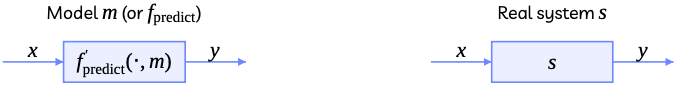
\includegraphics[width=0.7\textwidth]{assets/fig3.png}
    \caption{Model vs Real System}
\end{figure}

\definitionblock[Model vs Real System]{
    \begin{itemize}
        \item Collect examples of \textbf{s} behavior
        \item Feed \textbf{m} with examples 
        \item Compare responses of \textbf{s} and \textbf{m}
    \end{itemize}
    \textbf{Effectiveness:} to which degree the comparison step measures if m behaves like s.
}

\warningblock[$f_{collect}$]{
    The data collection is really important, since:
    \begin{itemize}
        \item small n $\to$ \textbf{poor} effectiveness, \textbf{great} efficiency
        \item large n $\to$ \textbf{good} effectiveness, \textbf{poor} efficiency
    \end{itemize}
    (effectiveness = accuracy, efficiency = resources)

    and also:
    \begin{itemize}
        \item poor coverage $\to$ \textbf{poor} effectiveness
        \item good coverage $\to$ \textbf{good} effectiveness
    \end{itemize}
    where coverage = how well the data represents the real system.
}

\begin{center}
    \begin{figure}[H]
        \centering
        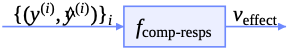
\includegraphics[width=0.5\textwidth]{assets/fig4.png}
        \caption{Comparing the responses}
    \end{figure}
\end{center}

where ${(y^{(i)}, \hat{y^{(i)}})}_i \in P^* (Y^2)$ is a multiset of pairs of y.

\exampleblock[Performance Indexes]{
    \textbf{Classification:}
    \begin{itemize}
        \item all types $\to$ error, accuracy 
        \item binary $\to$ EER, AUC, FPR, FNR and variants
        \item multi-class $\to$ weighted accuracy
    \end{itemize}
    \textbf{Regression:}
    \begin{itemize}
        \item MSE, MAE, R2
    \end{itemize}
}

\subsection{Classification}

In \inlinecode{Classification} Y is a finite set with no ordering.

The \textbf{Classification Error} is then 
\begin{center}
    $f_{err}({y^{(i)}, \hat{y^{(i)}}}) = \frac{1}{n}\sum_{i=1}^{i=n}\textbf{1}(y^{(i)} \neq \hat{y^{(i)}})$
\end{center}

where \textbf{1(b)} is the indicator function and takes value 1 when (in this case) the prediction is wrong.

The \textbf{Classification Accuracy} is instead:
\begin{center}
    $f_{acc}({y^{(i)}, \hat{y^{(i)}}}) = \frac{1}{n}\sum_{i=1}^{i=n}\textbf{1}(y^{(i)} = \hat{y^{(i)}})$
\end{center}

\textbf{Reminder:} $f_{acc} = 1 - f_{err}$

Extreme cases for accuracy (and errors) are:
\begin{itemize}
    \item m is s: \textbf{perfect model}
    \item m is random: does not model any dependence
\end{itemize}

\exampleblock[Random Classifier - Lower Bound]{
    $f_{random}(x) = y_i$ with $i ~ U({1, \dots, |Y|})$     just pick random uniformly
}
\exampleblock[Dummy Classifier - Better Lower Bound]{
    $f_{dummy}(x) = argmax \frac{1}{n} \sum_{i=1}^{i=n}\textbf{1}(y = y^{(i)})$     just pick the category with more example always
}
\exampleblock[Perfect Classifier - Upper Bound]{
    $f_{perfect}(x)= s(x)$
}
But the world is not deterministic, so a Bayes (stochastic) classifier may be better:
\exampleblock[Bayes Classifier - Better Upper Bound]{
    $f_{Bayes}(x) = argmax Pr(s(x) = y | x)$
}

\subsection{Binary Classification}

The main problem here are the \inlinecode{skewed datasets}, meaning the datasets with more example of a category than the other (we are considering only two categories here).

\definitionblock[FPR - False Positive Rate]{
    It is the rate of \textbf{negatives} that are wrongly classified as positives

    $FPR = \frac{FP}{N}$
}
\definitionblock[FNR - False Negative Rate]{
    It is the rate of positives that are wrongly classified as negatives.
    $FNR = \frac{FN}{P}$
}
Where
\begin{itemize}
    \item FP = False Positives 
    \item FN = False Negatives 
    \item P = Total positives 
    \item N = Total Negatives 
\end{itemize}

\begin{center}
    \begin{figure}[H]
        \centering
        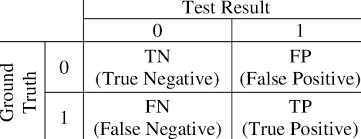
\includegraphics[width=0.5\textwidth]{assets/fig5.png}
        \caption{Confusion Matrix}
    \end{figure}
\end{center}

\inlinecode{TPR:} True Positive Rate = 1 - FNR

\inlinecode{FPR:} False Positive Rate = 1 - TNR

\inlinecode{Err:} Error Rate = $\frac{FP + FN}{P + N}$

\inlinecode{Acc:} Accuracy = $\frac{TP + TN}{P + N}$

\definitionblock[Balanced Data]{
    In classification, a dataset is \textbf{balanced} with respect to the response variable y, if the frequency of each value of y is roughly the same.
}

\inlinecode{Precision:} $\frac{TP}{TP + FP}$

\inlinecode{Recall:} $\frac{TP}{TP + FN}$

\inlinecode{F1:} $2 \cdot \frac{Precision \cdot Recall}{Precision + Recall}$

\inlinecode{Sensitivity:} $\frac{TP}{TP + FN} = TPR$

\inlinecode{Specificity:} $\frac{TN}{TN + FP} = TNR$

\inlinecode{Type I error:} False Positive Rate = FPR 

\inlinecode{Type II error:} False Negative Rate = FNR

\warningblock[Cost of the error]{
    Once $f_{predict}$ outputs a y, some action is taken, and if the action is wrong, there is some cost to be paid wrt the correct action.

    $c = c_{FP} \times FPR \times N + c_{FN} \times FNR \times P$

    If one knows the costs and N,P, it is possible to compute the overall cost and find a good trade-off for FPR and FNR.
}

Given a model, we can "tune" it to prefer avoiding FPs rather than FNs, just by modifying the threshold that is used to determine the choice to be made wrt the category.
Many learning techniques compute a probability distribution over Y before returning one y, and in the case of Binary Classification the threshold is 0.5. 

\begin{center}
    \begin{figure}[H]
        \centering
        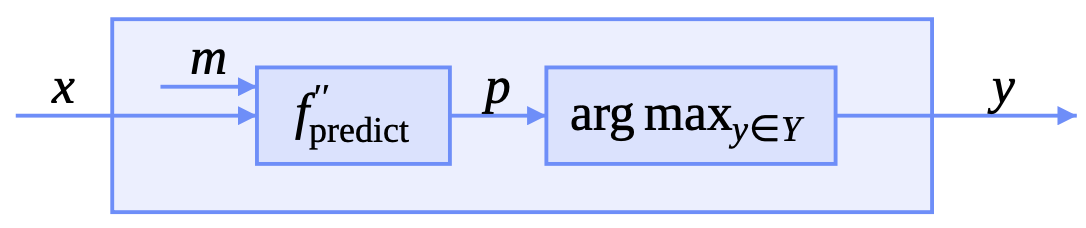
\includegraphics[width=0.5\textwidth]{assets/fig6.png}
        \caption{Threshold}
    \end{figure}
\end{center}
\newpage
So, by varying the threshold we can change FPR and FNR:
\begin{itemize}
    \item the greater the threshold, the lower FPR and the greater FNR
    \item the lower the threshold, the greater FPR and the lower FNR
\end{itemize}

\begin{center}
    \begin{figure}[H]
        \centering
        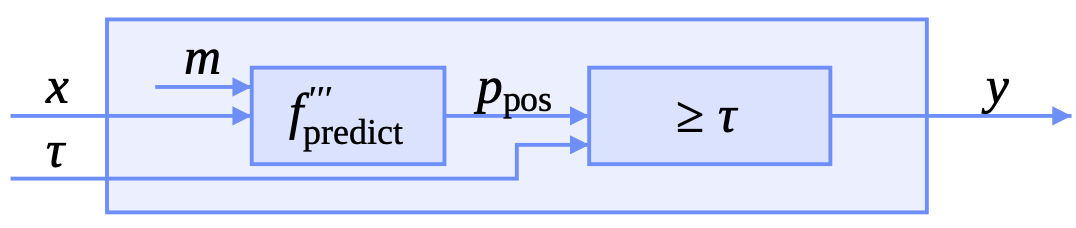
\includegraphics[width=0.5\textwidth]{assets/fig7.png}
        \caption{Threshold}
    \end{figure}
\end{center}

\definitionblock[ROC Curve (Receiver Operating Characteristic)]{
    The ROC curve is a graphical representation of the trade-off between the True Positive Rate (TPR) and the False Positive Rate (FPR) for every possible threshold.
}

\begin{center}
    \begin{figure}[H]
        \centering
        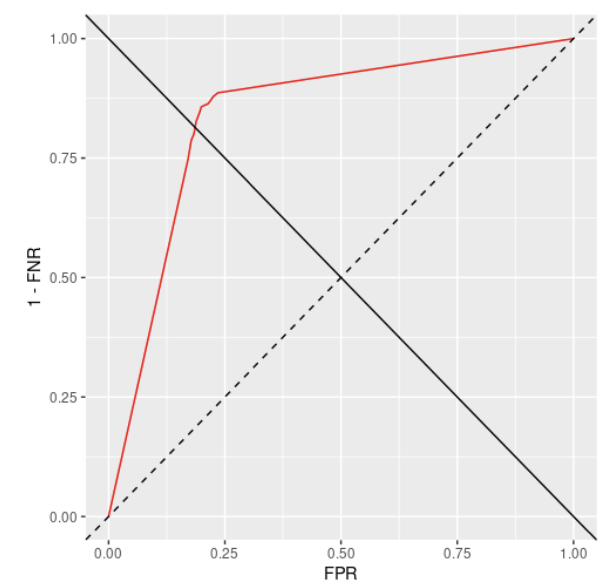
\includegraphics[width=0.5\textwidth]{assets/fig8.png}
        \caption{ROC Curve}
    \end{figure}
\end{center}

The dotted line represents the random classifier, while the closer the curve is to the top-left corner, the better the classifier is.

How to choose the threshold? Take different values and compute the ROC curve, then choose the one that is closer to the top-left corner. To do this, the best way is to take the \textbf{midpoints} of the sorted probabilities.

\newpage 

\subsection{Multiclass Classification and Regression}

Here we use the concept of \textbf{weighted accuracy}, which is 
    
    $f_{acc} = \frac{1}{|Y|}\sum_{y \in Y}^{}Acc_y$

\begin{figure}[H]
    \centering
    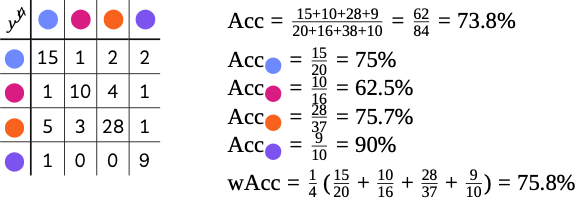
\includegraphics[width=0.5\textwidth]{assets/fig9.png}
    \caption{Multiclass Confusion Matrix}
\end{figure}

Moreover, the error there is different from the classification one: here we measure the \inlinecode{distance} from the real value.

\begin{itemize}
    \item \inlinecode{MAE:} Mean Absolute Error = $\frac{1}{n}\sum_{i=1}^{i=n}|y^{(i)} - \hat{y^{(i)}}|$
    \item \inlinecode{MSE:} Mean Squared Error = $\frac{1}{n}\sum_{i=1}^{i=n}(y^{(i)} - \hat{y^{(i)}})^2$   
    \item \inlinecode{RMSE:} Root Mean Squared Error = $\sqrt{MSE}$
    \item \inlinecode{MAPE:} Mean Absolute Percentage Error = $\frac{1}{n}\sum_{i=1}^{i=n}\frac{|y^{(i)} - \hat{y^{(i)}}|}{y^{(i)}}$
\end{itemize}

\subsection{Assessing Learning Techniques}
\begin{itemize}
    \item an \textbf{effective} learning technique is a pair of $f'_{learn}$, $f'_{predict}$ that learns a good model $m$
    \item a good \textbf{model} is one that has the same behavior of the real system $s$
\end{itemize}

We, then, want to measure the effectiveness of the learning techniques (learning and prediction).
To do so, we need to divide the dataset, since we want to see if the $f'_{predict}$ generalises well.

\definitionblock[Static Train/Test Division]{
    \begin{itemize}
        \item \textbf{Effectiveness:} generalization is assessed, but there is no robustness wrt D division 
        \item \textbf{Efficiency:} learning is executed only once 
    \end{itemize}
    $D_{test}$ is the unseen data and we treat is as said even if it has been collected at once with $D_{train}$.
}

\definitionblock[Repeated random train/test division]{
    \begin{itemize}
        \item \textbf{Effectiveness:} generalization is assessed, and there is robustness wrt D division 
        \item \textbf{Efficiency:} learning is executed multiple times \propto k
    \end{itemize}
}

\definitionblock[Cross-Validation]{
    \begin{itemize}
        \item \textbf{Effectiveness:} generalization is assessed, and there is robustness wrt D division 
        \item \textbf{Efficiency:} learning is executed multiple times \propto k
    \end{itemize}
}

\definitionblock[Leave-One-Out]{
    \begin{itemize}
        \item \textbf{Effectiveness:} generalization is assessed, and there is robustness wrt D division 
        \item \textbf{Efficiency:} learning is executed multiple times \propto n 
    \end{itemize}
    This is the worst case for efficiency, since we repeat the learning phase n times.
}

\begin{center}
    \begin{figure}[H]
        \centering
        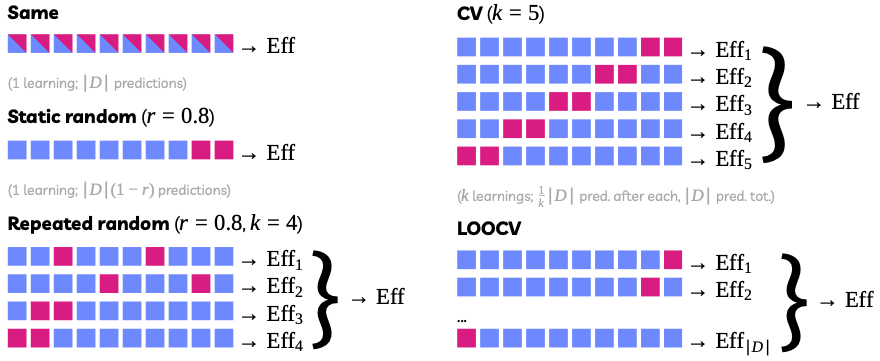
\includegraphics[width=0.8\textwidth]{assets/fig10.png}
        \caption{Train/Test Division Methods}
    \end{figure}
\end{center}

For comparison btw learning techniques, we can use the mean and standard deviation of the performance indexes obtained with the previous division methods. \textbf{Boxplots} are useful in this case.

\section{Tree-based Learning Techniques}

\subsection{Decision Trees}

A \textbf{Decision Tree} is a tree where each node is a decision on the value of a feature, and each branch is a possible value of the feature. The leaves are the categories. It can be understood in simpler terms by considering a basic \inlinecode{if-then-else} nested structure.

\begin{center}
    \begin{figure}[H]
        \centering
        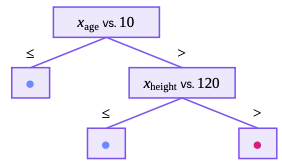
\includegraphics[width=0.5\textwidth]{assets/fig11.png}
        \caption{Decision Tree example}
    \end{figure}
\end{center}

This is a binary tree, but it can be n-ary as well. The tree is built by recursively splitting the dataset into subsets, and the splitting is done by selecting the feature that best splits the dataset into the purest subsets. The purity is measured by the \inlinecode{Gini Index} or the \inlinecode{Entropy}, usually.

One can also represent the tree in a compact way:
\begin{center}
    $t = [l, t', t'']$
\end{center}

where $l \in L$ is the \textbf{label} and $t', t'' \in T_L \cup \{\emptyset\}$ are the left and right children.

Also, each \textbf{non-terminal} node is a pair ($j, \tau$), where $j \in \{1, \dots, p\}$ is the index of the independent variable and $\tau \in R$ is the threshold for comparison.

The above figure is then represented as:

\begin{center}
    \begin{figure}[H]
        \centering
        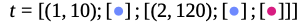
\includegraphics[width=0.5\textwidth]{assets/fig12.png}
        \caption{Compact representation of the Decision Tree}
    \end{figure}
\end{center}

\begin{center}
    \begin{algorithm}
        \caption{Templated $f'_{predict}$}
        function predict(x, t)\\
        \hspace{1cm} if \neg has-children(t) then return label(t)\\
        \hspace{1cm} else \{\\
            \hspace{2cm}(j, $\tau$) = label(t)\\
            \hspace{2cm}if x[j] $\leq \tau$ then return predict(x, left(t))\\
            \hspace{2cm}else return predict(x, right(t))\\
        \hspace{1cm}\}
    \end{algorithm}
\end{center}

This is a recursive function that works with every tree and always returnns a $y \in Y$.

\begin{center}
    \begin{figure}[H]
        \centering
        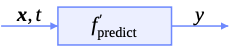
\includegraphics[width=0.5\textwidth]{assets/fig13.png}
        \caption{Templated $f'_{predict} : (R^p \times T_{p,Y}) \to Y$}
    \end{figure}
\end{center}

\warningblock[When to stop?]{
    The tree can grow indefinitely, so we need to stop it at some point. We can do this by:
    \begin{itemize}
        \item \textbf{Depth Limit:} stop when the depth is reached
        \item \textbf{Leaf Size:} stop when the leaf size is reached
        \item \textbf{Impurity:} stop when the impurity is below a certain threshold
    \end{itemize}
}

Also, how to find where to split the data? The algorithm searches for the best point wrt the accuracy, meaning it will find the point where accuracy (or misclassification to the contrary) is the best, that's why it is called \inlinecode{greedy}.

Other approaces are:
\begin{itemize}
    \item \textbf{Gini Index:} $Gini(t) = 1 - \sum_{y \in Y}^{}(Pr(y|t))^2$
    \item \textbf{Entropy:} $Entropy(t) = -\sum_{y \in Y}^{}Pr(y|t)log_2(Pr(y|t))$
\end{itemize}

They are both measures of impurity, and the best split is the one that minimizes the impurity. \textbf{The lower the better}.

\begin{center}
    \begin{figure}[H]
        \centering
        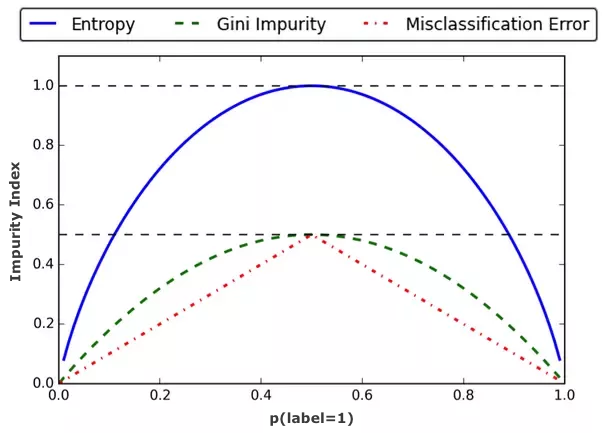
\includegraphics[width=0.5\textwidth]{assets/fig14.png}
        \caption{Gini Index, Entropy and Error}
    \end{figure}
\end{center}

Gini and Entropy are both smoother than the error, and they are similar, but Gini is faster to compute.

\subsection{Tree Learning with probabilities}

In this context terminal nodes \textbf{return discrete probability distributions}:

\begin{center}
    \begin{figure}[H]
        \centering
        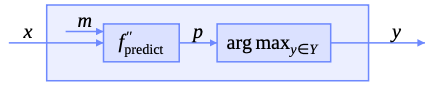
\includegraphics[width=0.5\textwidth]{assets/fig15.png}
        \caption{Tree Learning with probabilities}
    \end{figure}
\end{center}

\begin{center}
    $f''_{predict} : X_1 \times \dots \times X_p \times T_{(\{1, \dots, p\} \times R)\cup P_y}$
\end{center}

So the output will be the \inlinecode{frequency} of the categories.

\warningblock[Model Complexity]{
    Sometimes the tree could be too large wrt the real system. Almost every learning technique has at least one parameter that affects the maximum complexity of the learnable models, often called \textbf{flexibility}:
    \begin{itemize}
        \item more flexibility $\to$ more complex models
        \item less flexibility $\to$ simpler models
    \end{itemize}
}

The point is: the model tries to reach the maximum accuracy possible, but there is \inlinecode{noise} in the data, that leads to an impossible perfect score. 

\begin{center}
    \begin{figure}[H]
        \centering
        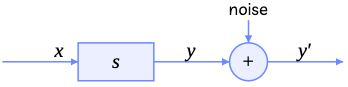
\includegraphics[width=0.5\textwidth]{assets/fig16.png}
        \caption{Noise in the data}
    \end{figure}
\end{center}

However, out goal is to \textbf{model s}, not $s+$noise.

\definitionblock[Overfitting]{
    When we have a \textbf{noisy dataset} and we allow for \textbf{large complexity}, by setting a flexibility parameter to a high flexibility, the learning technique \textbf{fits the noisy data} instead of the real system $s$, and \textbf{overfitting} occurs.
}

\textbf{Underfitting} is the opposite, when the model is too simple to capture the real system.

\begin{itemize}
    \item Underfitting exibits \textbf{high bias} and \textbf{low variance}, since it tends to generate models that incorporate a bias towards some y values 
    \item Overfitting, instead, exibits \textbf{low bias} and \textbf{high variance}, since it tends to generate different models if the learning is repeated with different datasets 
\end{itemize}

\exampleblock[Practical Procedure]{
    \begin{itemize}
        \item consider different values of the flexibility parameter
        \item choose a suitable \textbf{effectiveness index }
        \item choose a suitable \textbf{learning/testing division method} 
        \item learn a model and compute the performance index on the train and test set 
    \end{itemize}
}

\begin{center}
    \begin{figure}[H]
        \centering
        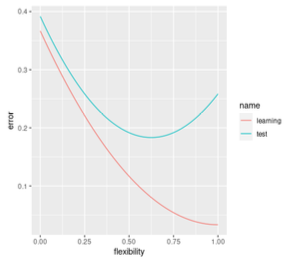
\includegraphics[width=0.4\textwidth]{assets/fig17.png}
        \caption{Bias-Variance Trade-off}
    \end{figure}
\end{center}

\definitionblock[Hyperparameter tuning]{
    It is the task of finding the tuple of hyperparameters $p^*_1, \dots, p^*_h \in P_j$ that maximizes the effectiveness index.
}

Hyperparameters are the parameters that are not learned by the learning technique, but are set by the user.

\exampleblock[Grid Search]{
    It is a simple form of hyperparameter tuning, where the user specifies a grid of values for each hyperparameter, and the learning technique is executed for each combination of hyperparameters. To be feasible, the set of hyperparameters must be small.
}

So why we can't just always use hyperparameter tuning instead of choosing a value? Well, it is expensive and probably lacks of generalization since it is specific fot that dataset.

\begin{center}
    \begin{figure}[H]
        \centering 
        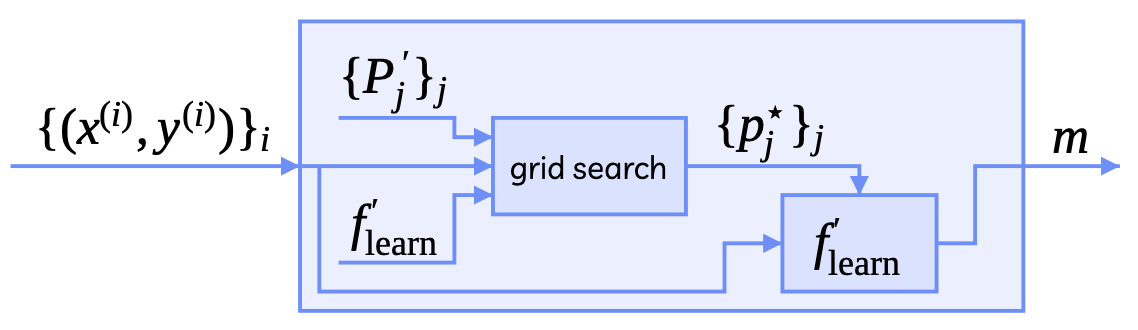
\includegraphics[width=0.5\textwidth]{assets/fig18.png}
        \caption{Hyperparameter-free Learning}
    \end{figure}
\end{center}

\subsection{Categorical Independent Variables and Regression}

Here we find a variable $x_j$ and a set of values $X'_j \in X_j$ that well separates the data. It's a simple binary split, where the $x_j$ is contained either in a group or the other.

\begin{center}
    \begin{figure}[H]
        \centering 
        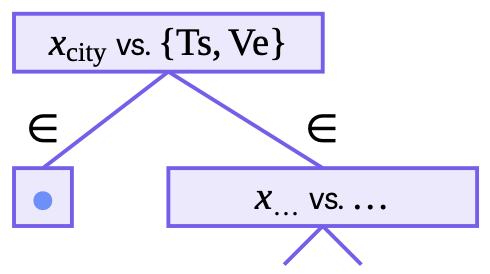
\includegraphics[width=0.3\textwidth]{assets/fig19.png}
        \caption{Tree with categorical variables}
    \end{figure}
\end{center}

For a given \textbf{categorical variable} $x_j \in X_j$, we choose $X'_j \subset X_j$ such that:

\begin{center}
    $X'_j = \operatorname*{argmin}_{X'_j \in P(X_j)} f_{impurity}(\{y^{(i)}\}_i |_{x^{(i)}_j \in X'_j}) + f_{impurity}(\{y^{(i)}\}_i |_{x^{(i)}_j \in X'_j})$
\end{center}

In a \textbf{Regression Tree}, instead, the terminal nodes are no more categorical values, they are instead numerical ones. For this reason concepts like $f_{impurity}$ or minimizing the error to stop do not hold anymore: they must be changed.

To find the best branch, RSS is the solution. 

\begin{center}
    $(j^*, \tau^*) = \operatorname*{argmin}_{j, \tau} RSS(\{y^{(i)}\}_i |_{x^{(i)}_j \leq \tau}) + RSS(\{y^{(i)}\}_i |_{x^{(i)}_j \leq \tau})$
\end{center}

Also for the \textbf{Stopping Criterion}, we should use RSS instead of the error, then stopping when $RSS=0$ or when $n \leq n_{min}$. To notice that $RSS=0$ is much more unfrequent than error$=0$.

\begin{center}
    \begin{figure}[H]
        \centering 
        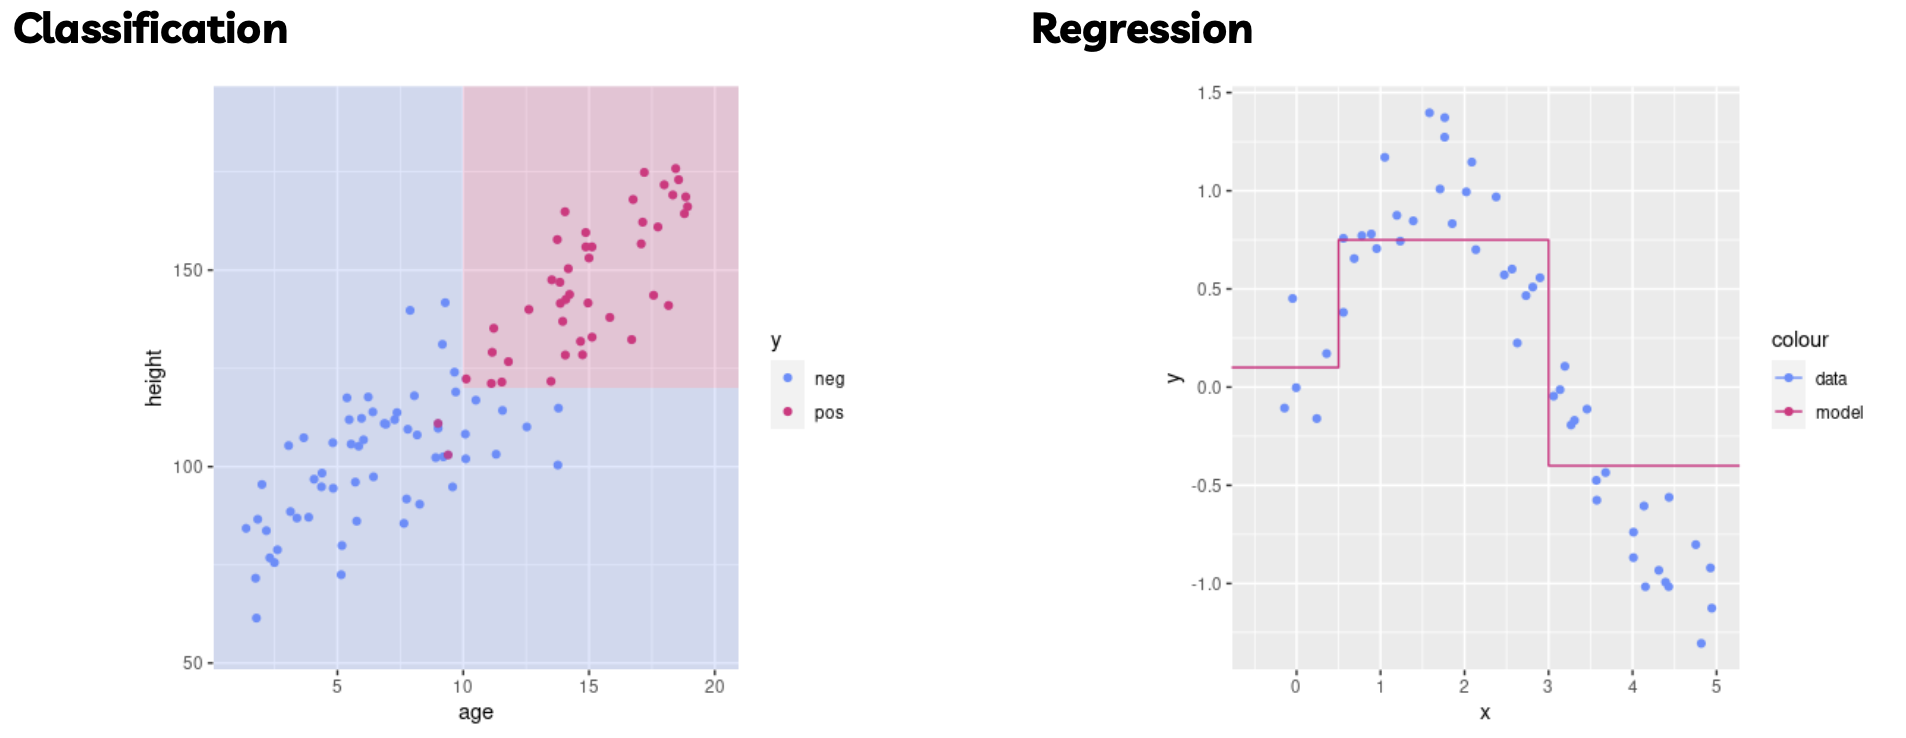
\includegraphics[width=1\textwidth]{assets/fig20.png}
        \caption{Classification Tree vs Regression Tree}
    \end{figure}
\end{center}

\section{Tree Bagging and Random Forest}

\subsection{Tree Bagging}

If we learn a regression tree with \textbf{low flexibility}:
\begin{itemize}
    \item the model will not capture the system behavior 
    \item it will underfit the data and the system 
\end{itemize}
If we learn a regression tree with \textbf{high flexibility}:
\begin{itemize}
    \item the model will likely better capture the system behavior, but\dots
    \item it will model also some noise
    \item it will overfit the data 
\end{itemize}

\inlinecode{What if we combine the power of the high flexibility obtained from different models?}

\definitionblock[Wisdom of the crowds theorem]{
    A collective opinion may be better than a single expert's opinion
}

\warningblock[Wisdom of the crowds theorem]{
    Yes, but only if:
    \begin{itemize}
        \item we have many opinions \to (learn many trees)
        \item they are independent \to (each tree is learned on a dataset obtained with sampling with repetition)
        \item we have a way to aggregate them \to (aggregate the predictions)
    \end{itemize}
}

For the \textbf{independency} part, we just have to use \inlinecode{different learning sets}, using for example the Cross-Validation technique or, even better, the Bootstrap technique.

\begin{center}
    \begin{figure}[H]
        \centering
        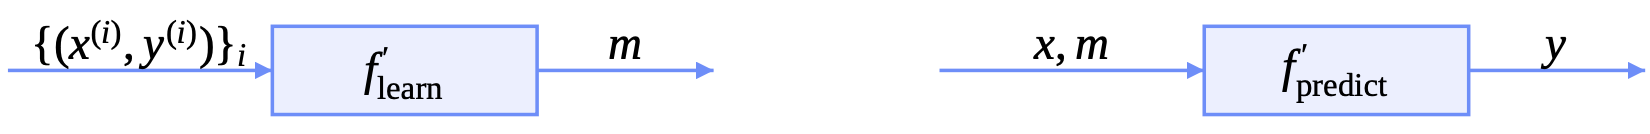
\includegraphics[width=1\textwidth]{assets/fig21.png}
        \caption{Tree bagging}
    \end{figure}
\end{center}

\definitionblock[Tree Bagging]{
    \begin{itemize}
        \item \textbf{Learning:} the model is a bag of trees and we can specify the number of trees as an hyperparameter. Remember that the learning technique is not deterministic due to the random sampling part.
        \item \textbf{Predict:} for classification consider the majority of votes for every $y \in Y$ (label), for regression simply return the mean of the relative values (better if also the $\sigma$ is returned, to have a measure of the uncertainty)
    \end{itemize}
}

\warningblock[$n_{tree} hyperparameter$]{
    It is a flexibility parameter, but if increased changes overfitting and generalisation in the same way. Experimentally turns out 
    that with a reasonably large $n_{tree}$ bagging is better than single tree learning, and after that number there is no tendency to overfit.
    The problem is that the higher the parameter, the less efficient is the model. Simple trade-off.
}

\subsection{Random Forest}

The question is: can we further increase the independency such that the model will possibly learn different patterns in the data? The answer is yes, and we can do it by including more independency not only in the learning set, but also in the way the learning technique chooses the predictors each time. A sort of \textbf{independency in the predictors' sets}.

\textbf{Idea:} when learning each tree, \textbf{remove some randomly chosen independent variables} from the observations. This is called \textbf{Random Forest}, and is a learning technique that enhances the capabilities of Tree Bagging with variables removal.
\begin{itemize}
    \item \textbf{Random:} because there are two sources of randomness, hence of independency
    \item \textbf{Forest:} because it gives a bag of trees 
\end{itemize}

\begin{center}
    \begin{figure}[H]
        \centering 
        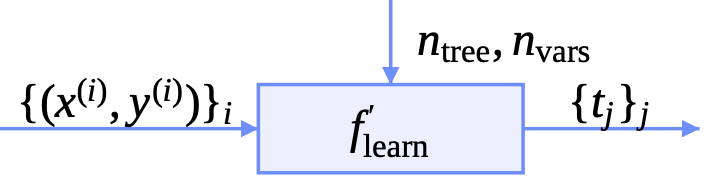
\includegraphics[width=0.5\textwidth]{assets/fig22.png}
        \caption{Random Forest}
    \end{figure}
\end{center}

The model is a bag of $n_{vars}$ trees, as in bagging, where that parameter is $\leq p$ that is the number of variables. Two parts of this learning technique are \textbf{not deterministic}: where it samples observations to create the various learning sets for the various trees and where it chooses the predictors to use.

For prediction just refer to bagging, it is the same.

Is the fact that not all predictors are uses in each tree a problem? Well, no. The model still considers all the predictors but chooses not to use some of them.

\warningblock[Random Forest]{
    The opposite, i.e. when the variable is in the tree but valued not in x, is a problem.
}

Experimentally turns out that $n_{vars}$ does not impact the tendency to overfit, hence it is not a proper flexibility parameter. 
Good default values are:
\begin{itemize}
    \item $\sqrt{p}$ for classification 
    \item $\frac{1}{3}p$ for regression 
\end{itemize}

For this reason (remember that also $n_tree$ does not impact overfitting) Random Forest is almost a \textbf{hyperparameter-free learning technique!} (\to just use default values)

\begin{center}
    \begin{figure}[H]
        \centering 
        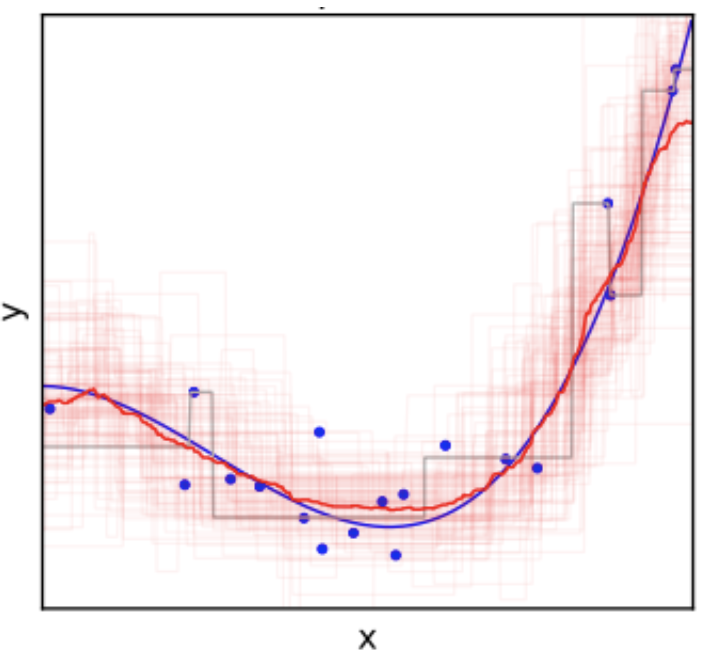
\includegraphics[width=0.4\textwidth]{assets/fig23.png}
        \caption{Random Forest}
    \end{figure}
\end{center}

\definitionblock[OOB error]{
    This value is computed on the unseen observations at each step of the ensemble.
    \begin{itemize}
        \item For each observation, find the out-of-bag trees and obtain their prediction on the observations
        \item compute the error on the predictions 
    \end{itemize}
    To remark that this is an \textbf{estimate} of the test error, but does not need a test dataset and is computed at learning time.
}

\begin{center}
    \begin{figure}[H]
        \centering 
        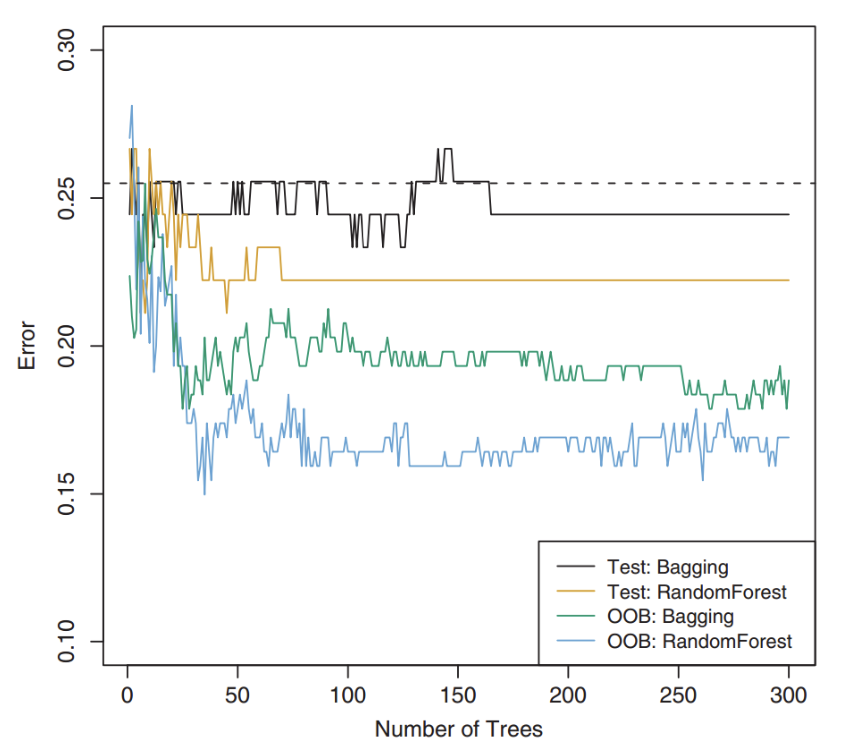
\includegraphics[width=0.38\textwidth]{assets/fig24.png}
        \caption{Error}
    \end{figure}
\end{center}
\warningblock[Interpretability]{
    Ensemble methods lack of Interpretability, since they consider different scenarios and use the computational power to find human-invisible patterns in the data.
}

\textbf{Variable importance:} compute teh RSS/Gini before and after each branch-node and assign the increase/decrease to the branch-node variable; this way a ranking of variables can be created (the larger, the more important).

But this process is not so effective, since tends to prefer numerical variables and works with learning data. 

A better option is the \textbf{mean accuracy decrease}, just after learning.
\begin{enumerate}
    \item for each j-th variable and each tree t in the bag 
    \begin{enumerate}
        \item take the observations in $D_t$ not used for t 
        \item measure the accuracy of t on $D_t$
        \item shuffle the j-th variable in the observations, obtaining $D'_t$
        \item measure again the accuracy 
        \item assigne the decrease in accuracy to the j-th variable 
    \end{enumerate}
    \item build a ranking of variables based on the sum of decreases (the larger, the more important)
\end{enumerate}

\textbf{Rationale:} if the decrease is low, shuffling the variable has no meaning (variable is not so important).

A more general approach comes with \textbf{feature ablation}:
\begin{enumerate}
    \item measure the effectiveness of $f'_{learn}, f'_{predict}$ on the dataset D 
    \item for each j-th variable $x_j$
    \begin{enumerate}
        \item build a D' by removing $x_j$ from D 
        \item measure the effectiveness of $f'_{learn}, f'_{predict}$ on D' 
        \item compute the j-th variable importance as the decrease of effectiveness in D' wrt D 
    \end{enumerate}
    \item build a ranking of variables based on the decrease in effectiveness (as always, the larger, the more important)
\end{enumerate}

Here some variables are removed to see what happens.

\definitionblock[No free lunch theorem]{
    Any two optimization algorithms are equivalent when their performance is averaged across all possible problems
}

\section{Support Vector Machines}

The learning techniques seen before lack of usefulness in some types of datasets, like the below one:

\begin{center}
    \begin{figure}[H]
        \centering
        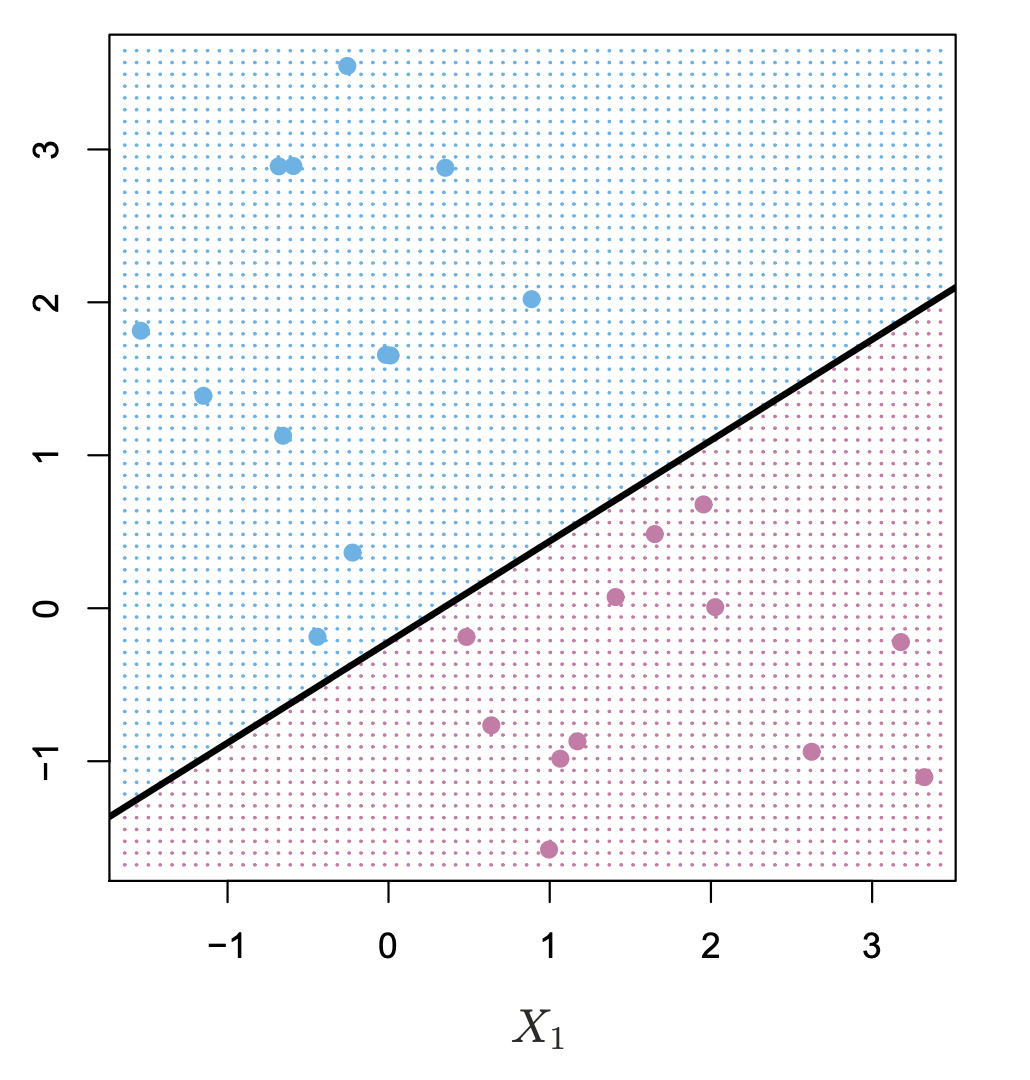
\includegraphics[width=0.4\textwidth]{assets/fig25.png}
    \end{figure}
\end{center}

Here, an \textbf{Hyperplane} can be used to tella apart the points with different labels. SVM are intended for the binary classification setting in which there are two classes.

\definitionblock[Hyperplane]{
    In a p-dimensional space, a hyperplane is a flat affine subspace of dimension $p-1$. 
    \begin{center}
        $\beta_0 + \beta^T_x = 0$
    \end{center}
    Since it divides the space in two parts, if the data is contained in one subspace it will be classified as $y_1 \in Y$, otherwise as $y_2 \in Y$.
}

\begin{center}
    \begin{figure}[H]
        \centering
        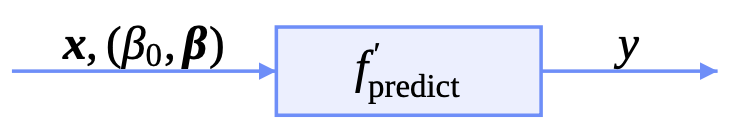
\includegraphics[width=0.5\textwidth]{assets/fig26.png}
        \caption{SVM $f_{predict}$}
    \end{figure}
\end{center}

\textbf{Assumptions:}
\begin{itemize}
    \item Y = Pos,Neg $\to$ binary classification only!
    \item X $= R^{p}$ $\to$ numerical independent variables only!
\end{itemize}

It is computationally very fast, since there are just p multiplications and sums.

The \inlinecode{magnitude} of a vector of predictors is the distance from the hyperplane, meaning that the greater the magnitude, the more the point is far from the hyperplane and the more confident is the prediction.

But, how to choose the best hyperplane?

\begin{center}
    \begin{figure}[H]
        \centering
        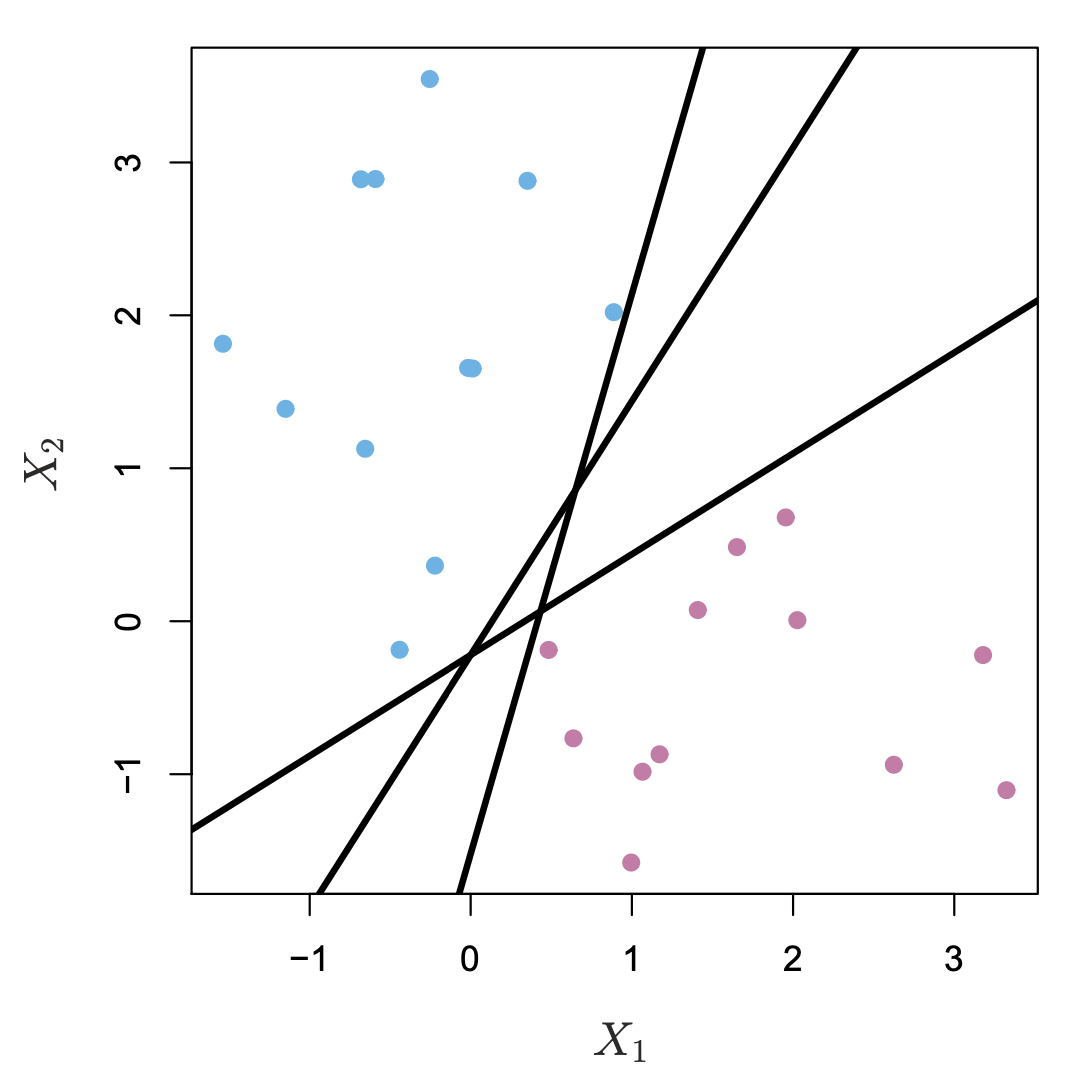
\includegraphics[width=0.4\textwidth]{assets/fig27.png}
    \end{figure}
\end{center}

\definitionblock[Maximal Margin Hyperplane]{
    The best hyperplane is the one that maximizes the distance from the closest point to the hyperplane. This distance is called \textbf{margin} and is the (perpendicular) distance from each training observation to a given separating hyperplane; the smallest such distance is the minimal distance from the observations to the hyperplane.
    The maximal margin hyperplane is the separating hyperplane for which the margin is largest,that is, it is the hyperplane that has the farthest minimum distance to the training observations.
}

\begin{center}
    \begin{figure}[H]
        \centering
        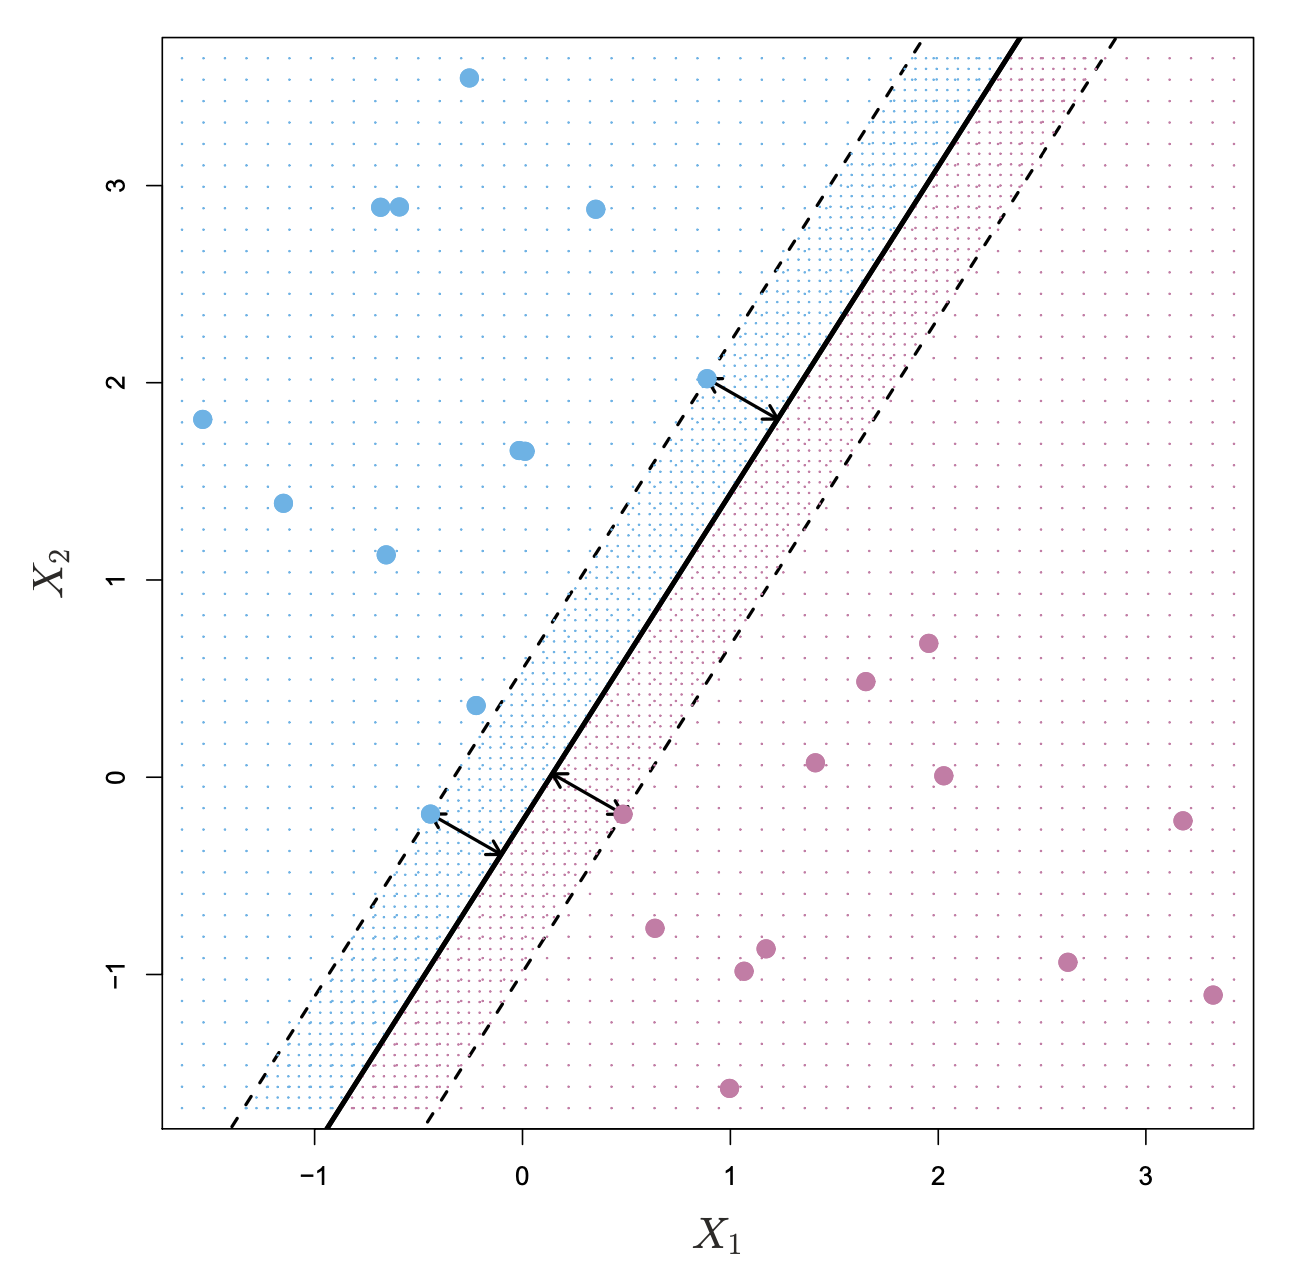
\includegraphics[width=0.4\textwidth]{assets/fig28.png}
        \caption{Maximal Margin Hyperplane}
        \label{fig:hyperplane2}
    \end{figure}
\end{center}

In fig.\ref{fig:hyperplane2} three training observations are equidistant from the maximal margin hyperplane and lie along the dashed lines indicating the width of the margin. These three observations are known as support vectors,since they are vectors in p-dimensional space and they “support” the maximal margin hyperplane in the sense that if these points were moved slightly then the maximal margin hyperplane would move as well.

How to learn an hyperplane:
\begin{itemize}
    \item must perfectly separates the data
    \item must maximize the margin
\end{itemize}

It is an optimization problem, searching for the best $m$ with the constraint that every point must be on the proper size and at a distance $\geq m$ from the hyperplane.

\warningblock[Applicability]{
    What if some noise is introduced in the predictors? The \textbf{support vectors} change just a bit and the hyperplane changes as well, it can even not exist anymore! \textbf{Tolerance} must be introduced.
}

\definitionblock[Soft Margin Classifier]{
    \begin{itemize}
        \item $\operatorname*{argmax}_{\beta_0 \dots \beta_p, \epsilon^(1) \dots \epsilon^(n)}$ m 
        \item subject to $\sum_{j=1}^{j=p}\beta_j^2 = \beta \beta^T = 1$
        \item $y^{(i)}(\beta_0 + \beta^T x^{(i)}) \geq m(1 - \epsilon^{(i)}) \forall i = 1 \dots n$
        \item $\epsilon^{(i)} \geq 0 \forall i = 1 \dots n$
        \item $\sum_{i=1}^{n} \epsilon^{(i)} = c$
    \end{itemize}
    $\epsilon^{(1)} \dots \epsilon^{(i)}$ are positive slack variables: they act as tolerance wrt the margin.
    
    Due to the tolerance (c), the margin can be pushed. $c \in R^+$ is a budget of tolerance.
}

\textbf{c} is a flexibility parameter:
\begin{itemize}
    \item $c = \infty$ \to infinite tolerance, you can move a lot the points and the line stay the same hence the model is the same irrespective of learning data (\textbf{high bias})
    \item $c = 0$ \to no tolerance, the model is the best wrt the learning data but it is not generalizable (\textbf{high variance})
\end{itemize}

\textbf{Variable scale} plays an important role here, since we are computing a matrix multiplication and the high coefficients' difference can be subject to noise. For this reason, the data must be \textbf{standardized}:
\begin{itemize}
    \item \textbf{min-max scaling}: $x^{(i)}_j = \frac{x^{(i)}_j - \operatorname*{min}_i x^{(i')}_j}{\operatorname*{max}_i x^{(i')}_j - \operatorname*{min}_i x^{(i')}_j}$
    \item \textbf{standardization}: $\frac{1}{\sigma_j} (x^{(i)}_j - \mu_j)$
\end{itemize}

Since scaling must be done both in learning and in prediction, the coefficients needed for scaling do \textbf{belong to the model}.

\begin{center}
    \begin{figure}[H]
        \centering
        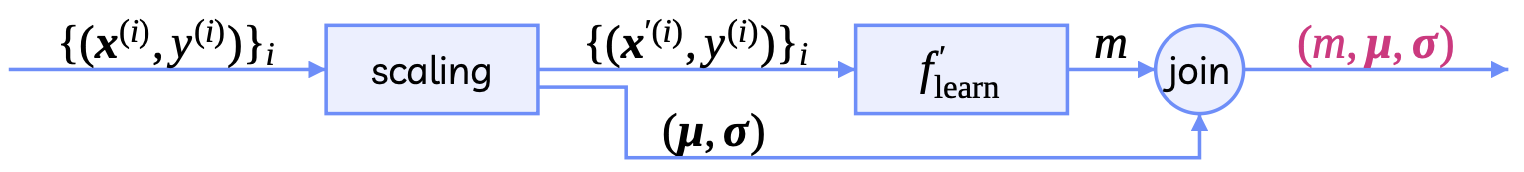
\includegraphics[width=0.7\textwidth]{assets/fig29.png}
        \caption{Learning with standardization}
    \end{figure}
\end{center}

\begin{center}
    \begin{figure}[H]
        \centering
        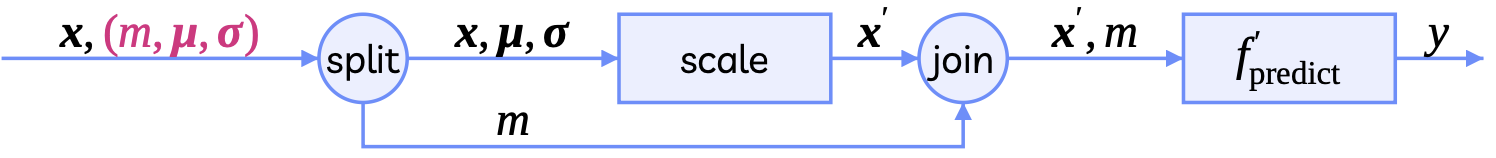
\includegraphics[width=0.7\textwidth]{assets/fig30.png}
        \caption{Prediction with standardization}
    \end{figure}
\end{center}

Another formulation for the tolerance is the following:
\begin{itemize}
    \item $\operatorname*{max}_{\beta_0,\dots,\beta_p,\epsilon^{(1)},\dots,\epsilon^{(i)}} m - c\sum_{i=1}^{n}\epsilon^{(i)}$
    \item subject to the previous constraints
\end{itemize}

Regarding c, it is a weighting factor that balances the trade-off between the margin and the tolerance. It is a flexibility parameter, and it is usually set by the user.
\begin{itemize}
    \item $c = 0 \to$ points that are inside the margin cost zero, you can put the line wherever you want, the model is always the same (\textbf{high bias})
    \item $c = \infty \to$ points that are inside the margin cost infinite, the model is the best wrt the learning data but it is not generalizable (\textbf{high variance})
\end{itemize}

\warningblock[Differences between SMCs]{
    There is one learning parameter c, it is a flexibility parameter.
    \textbf{Differences}:
    \begin{itemize}
        \item c extreme values:
        \begin{itemize}
            \item $c = +\infty$ (1st) and $c = 0$ (2nd) $\to$ high bias 
            \item $c = 0$ (1st) and $c = +\infty$ (2nd) $\to$ high variance
        \end{itemize}
        \item learnability:
        \begin{itemize}
            \item with the 2nd, a model can \textbf{always} be learned 
            \item with the 1st, there is a $c \leq 0$ such that a c value lower than that leads to an impossibility to learn a model from D 
        \end{itemize}
    \end{itemize}
}

\definitionblock[Kernel]{
    We can formuate alternatilvely the $f'_{predict}$ in this way:
    \begin{center}
        $f'_{predict}(x) = \beta_0 + \sum_{i=1}^{n}\alpha^{(i)}K(x, x^{(i)})$
    \end{center}
    where $K(x, x^{(i)})$ is the kernel function, that is a function that computes the similarity between two points.

    The idea behind this function is to:
    \begin{itemize}
        \item transform the data in a higher-dimensional space ($X = R^p \to X = R^q$) and then 
        \item compute the inner product in the destination space, i.e., $k(x,x^{(i)}) = \phi(x^T)\phi(x^{(i)})$
    \end{itemize}
    hoping that an hyperplane in the destination space is a non-linear hyperplane in the original space.
}

When using a kernel function, the learing technique is called \inlinecode{Support Vector Machines}.

\exampleblock[Common Kernel Functions]{
    \begin{itemize}
        \item \textbf{Linear Kernel:} $K(x, x^{(i)}) = x^T x^{(i)}$, the most efficient and computationally cheapest
        \item \textbf{Polynomial Kernel:} $K(x, x^{(i)}) = (x^T x^{(i)} + 1)^d$, where d is the degree of the polynomial
        \item \textbf{Radial Basis Function (RBF) Kernel:} $K(x, x^{(i)}) = exp(-\gamma ||x - x^{(i)}||^2)$, where $\gamma$ is a flexibility parameter, this is the most widely used 
    \end{itemize}
}

\textbf{Intuition of RBF:} it maps an x to the space where coordinates are the distances to relevant observations of the learning data. In practice, the decision boundary can smoothly follor any path (with risk of overfitting).

\begin{center}
    \begin{figure}[H]
        \centering
        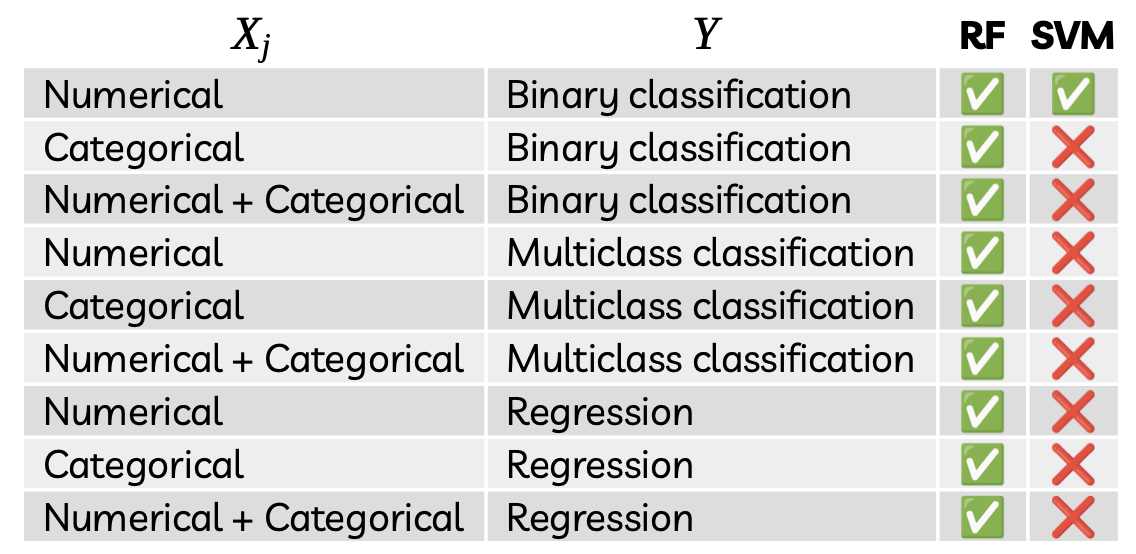
\includegraphics[width=0.5\textwidth]{assets/fig31.png}
        \caption{Applicability?}
    \end{figure}
\end{center}

How can improve the SVM applicability to other types of data?

\definitionblock[Encoding]{
    The idea is to encode the data in a way that the SVM can learn a model from it. This is done by:
    \begin{itemize}
        \item \textbf{One-Hot Encoding:} for categorical variables, each category is transformed in a binary variable, increasing the number of predictors
        \item \textbf{Ordinal Encoding:} for ordinal variables, each category is transformed in a numerical variable
    \end{itemize}
}
\newpage
\textbf{One-vs-One}

Technique to extend the SVM to multiclass classification. The idea is to learn a binary classifier for each pair of classes, and then to use a voting system to classify the new data. $\to M^{\frac{k(k-1)}{2}}$ 

\textbf{One-vs-All}

Technique to extend the SVM to multiclass classification. The idea is to learn a binary classifier for each class, and then to use a voting system to classify the new data. $\to M^k$

\warningblock[Missing Values]{
    \begin{itemize}
        \item drop the relative observations
        \item drop the relative predictors
        \item impute the missing values
    \end{itemize}
}

\section{Naive Bayes}

This learning techniques utilizes the \textbf{Bayes' Theorem} to classify the data. It is a probabilistic approach, and it is based on the assumption that the predictors are independent. Here there are the concepts of \textbf{prior probability} and \textbf{posterior probability}.

\begin{center}
    $Pr(A|B) = \frac{Pr(A)Pr(B|A)}{Pr(B)}$
\end{center}

where:
\begin{itemize}
    \item $Pr(A|B)$ is the posterior probability
    \item $Pr(A)$ is the prior probability
    \item $Pr(B|A)$ is the likelihood
    \item $Pr(B)$ is the evidence
\end{itemize}

Assumptions:
\begin{itemize}
    \item X = $X_1 \times \dots \times X_p$
    \item Y = \{$y_1, \dots, y_k$\}
\end{itemize}

\definitionblock[Naive Bayes]{
    \begin{itemize}
        \item \textbf{Learning:} the model is a set of conditional probabilities, one for each predictor and each category
        \item \textbf{Predict:} for each category, compute the product of the conditional probabilities and the prior probability, then choose the category with the highest value
    \end{itemize}
}

Hence, $p(y_m | x_{1,l_1},\dots,x_{p,l_p}) = p(y_m)\frac{p(x_{1,l_1},\dots,x_{p,l_p} | y_m)}{p(x_{1,l_1},\dots,x_{p,l_p})}$

In the \textbf{Naive} approach, where the predictors are independent, it becomes:

$p(y_m | x_{1,l_1},\dots,x_{p,l_p}) = \frac{p(y_m)}{p(x_{1,l_1},\dots,x_{p,l_p})}p(x{1,l_1} | y_m) \dots p(x_{p,l_p} | y_m)$

that can be found in the dataset.

\begin{center}
    \begin{figure}[H]
        \centering
        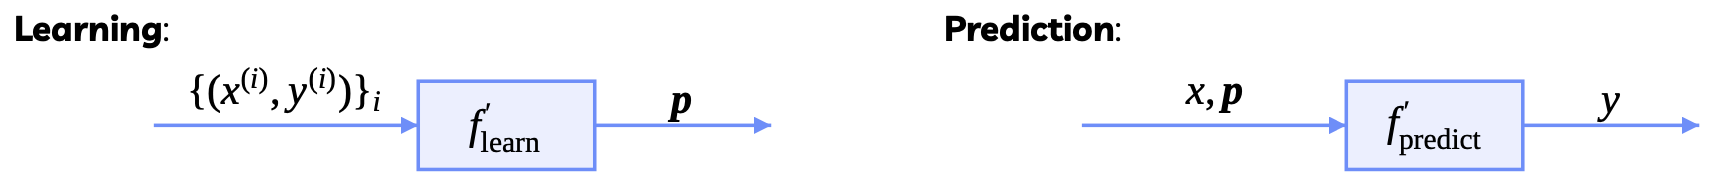
\includegraphics[width=1\textwidth]{assets/fig32.png}
        \caption{Naive Bayes}
    \end{figure}
\end{center}

The model p is some data structure holding $k + \sum_{j=1}^{p}kh_j$ numbers.

\section{k-Nearest Neighbors (KNN)}

This learning technique is based on the idea that similar data points are close to each other in the space. The model is the dataset itself, and the learning technique is just a function that computes the distance between the new data and the dataset.

\begin{center}
    \begin{figure}[H]
        \centering
        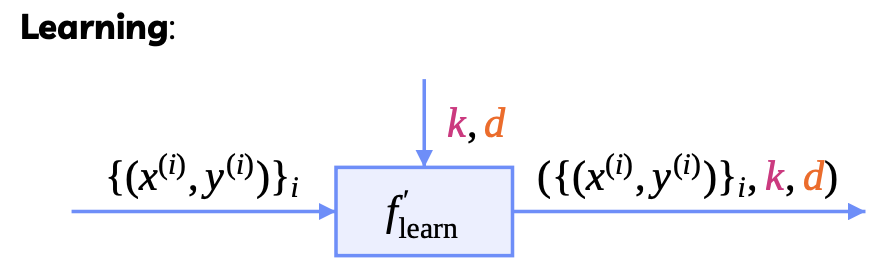
\includegraphics[width=0.8\textwidth]{assets/fig33.png}
    \end{figure}
\end{center}

$f'_{learn}$ does nothing, $f'_{predict}$ computes the distance between the new data and the dataset, then selects the k-nearest neighbors and returns the majority class. k and d are parameters!

\begin{center}
    \begin{figure}[H]
        \centering
        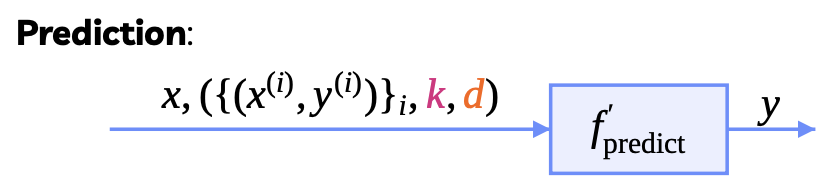
\includegraphics[width=0.8\textwidth]{assets/fig34.png}
    \end{figure}
\end{center}

For regression, return $\frac{1}{k}\sum_{i \in I}y^{(i)}$

With the proper distance function, the KNN can be used for any type of data.

\exampleblock[Common distance functions]{
    \begin{itemize}
        \item \textbf{Euclidean Distance:} $d(x, x^{(i)}) = \sqrt{\sum_{j=1}^{p}(x_j - x^{(i)}_j)^2}$
        \item \textbf{Manhattan Distance:} $d(x, x^{(i)}) = \sum_{j=1}^{p}|x_j - x^{(i)}_j|$
        \item \textbf{Minkowski Distance:} $d(x, x^{(i)}) = (\sum_{j=1}^{p}|x_j - x^{(i)}_j|^q)^{\frac{1}{q}}$
    \end{itemize}
}

k is a flexibility parameter, and it is usually set by the user. It is a trade-off between bias and variance:   
\begin{itemize}
    \item $k = 1$ \to high variance, low bias
    \item $k = n$ \to high bias, low variance
\end{itemize}


